%from module 5-1 pg 163
\subsection{Causal Reasoning}
Inductive arguments are used to support claims about cause and effect. These arguments come in
a number of different forms. The most straightforward is what is called enumerative induction.
This is an argument that makes a (non-hasty) generalization, inferring that one event or type of
event causes another on the basis of a (large) number of particular observations of the cause
immediately preceding the effect. To use a very famous example (from the history of philosophy,
due to David Hume, the 18th century Scottish philosopher who had much to say about cause and
effect and inductive reasoning), we can infer from observations of a number of billiard-ball
collisions that the first ball colliding with the second causes the second ball to move. Or we can
infer from a number of observations of drunkenness following the consumption of alcoholic
beverages that imbibing alcohol causes one to become drunk.

This is all well and good, so far as it 
goes.\footnote{Setting aside Hume's philosophical skepticism about our ability to know that one thing 
causes another and about the
conclusiveness of inductive reasoning.}
It just doesn't go very far. If we want to establish a
robust knowledge of what causes the natural phenomena we're interested in, we need techniques
that are more sophisticated than simple enumerative induction. There are such techniques. These
are patterns of reasoning identified and catalogued by the 19th century English philosopher,
scientist, logician, and politician John Stuart Mill. The inferential forms Mill enumerated have
come to be called ``Mill's Methods'', because he thought of them as tools to be used in the
investigation of nature--methods of discovering the causes of natural phenomena. In this section,
we will look at Mill's Methods each in turn (there are five of them), using examples to illustrate
each. We will finish with a discussion of the limitations of the methods and the difficulty of
isolating causes.

\subsubsection{The Meaning(s) of `Cause'}
Before we proceed, however, we must issue something of a disclaimer: when we say the one action
or event causes another, we don't really know what the hell we're talking about. OK, maybe that's
putting it a bit too strongly. The point is this: the meaning of `cause' has been the subject of intense
philosophical debate since ancient times (in both Greece and India)--debate that continues to this
day. Myriad philosophical theories have been put forth over the millennia about the nature of
causation, and there is no general agreement about just what it is (or whether causes are even real!).

We're not going to wade into those philosophical waters; they're too deep. Instead, we'll merely
dip our toes in, by making a preliminary observation about the word `cause'--an observation that
gives some hint as to why it's been the subject of so much philosophical deliberation for so long.
The observation is this: there are a number of distinct, but perfectly acceptable ways that we use
the word `cause' in everyday language. We attach different incompatible meanings to the term in
different contexts.

Consider this scenario: I'm in my backyard vegetable garden with my younger daughter (age 4 at
the time). She's ``helping'' me in my labors by watering some of the 
plants.\footnote{Those who have ever employed a 4-year-old to facilitate a labor-intensive project will 
understand the scare quotes.}
She asks, ``Daddy,
why do we have to water the plants?'' I might reply, ``We do that because water causes the plants
to grow.'' This is a perfectly ordinary claim about cause and effect; it is uncontroversial and true.
What do I mean by `causes' in this sentence? I mean that water is a necessary condition for the
plants to grow. Without water, there will be no growth. It is not a 
sufficient condition for plantgrowth, though: you also need sunlight, good soil, etc.

Consider another completely ordinary, uncontroversial truth about causation: decapitation causes
death. What do I mean by `causes' in this sentence? I mean that decapitation is a sufficient
condition for death. If death is the result you're after, decapitation will do the trick on its own;
nothing else is needed. It is not (thank goodness) a necessary condition for death, however. There
are lots of other ways to die besides beheading.

Finally, consider this true claim: smoking causes cancer. What do I mean by `causes' in this
sentence? Well, I don't mean that smoking is a sufficient condition for cancer. Lots of people
smoke all their lives but are lucky enough not to get cancer. Moreover, I don't mean that smoking
is a necessary condition for cancer. Lots of people get cancer--even lung cancer--despite having
never smoked. Rather, what I mean is that smoking tends to produce cancer, that it increases the
probability that one will get cancer.

So, we have three totally ordinary uses of the word `cause', with three completely different
meanings: cause as necessary condition, sufficient condition, and mere tendency (neither necessary
nor sufficient). These are incompatible, but all acceptable in their contexts. We could go on to list
even more uses for the term, but the point has been made. Causation is a slippery concept, which
is why philosophers have been struggling for so long to capture its precise meaning. In what
follows, we will set aside these concerns and speak about cause and effect without hedging or
disclaimers, but it's useful to keep in mind that doing so papers over some deep and difficult
philosophical problems.

\subsubsection{Mill's Methods}
John Stuart Mill identified five different patterns of reasoning that one could use to discover
causes. These are argument forms, the conclusions of which involve a claim to the effect that one
thing causes (or is causally related to) another. They can be used alone or in combination,
depending on the circumstances. As was the case with analogical reasoning, these are patterns of
inference that we already employ unreflectively in everyday life. The benefit in making them
explicit and subjecting them to critical scrutiny is that we thereby achieve a metacognitive
perspective--a perspective from which we can become more self-aware, effective reasoners. This
is especially important in the context of causal reasoning, since, as we shall see, there are many
pitfalls in this domain that we a prone to fall into, many common errors that people make when
thinking about cause and effect.

\paragraph{Method of Agreement}

I've been suffering from heartburn recently. Seems like at least two or three days a week, by about
dinnertime, I've got that horrible feeling of indigestion in my chest and that yucky taste in my
mouth. Acid reflux: ugh. I've got to do something about this. What could be causing my heartburn,
I wonder? I know that the things you eat and drink are typical causes of the condition, so I start
thinking back, looking at what I've consumed on the days when I felt bad. As I recall, all of the
recent days on which I suffered heartburn were different in various ways: my dinners ranged from
falafel to spaghetti to spicy burritos; sometimes I had a big lunch, sometimes very little; on some
days I drank a lot of coffee at breakfast, but other days not any at all. But now that I think about it,
one thing stands out: I've been in a nostalgic mood lately, thinking about the good old days, when
I was a carefree college student. I've been listening to lots of music from that time, watching old
movies, etc. And as part of that trip down memory lane, I've re-acquired a taste for one of my
favorite beverages from that era--Mountain Dew. I've been treating myself to a nice bottle of the
stuff with lunch now and again. And sure enough, each of the days that I got heartburn was a day
when I drank Mountain Dew at lunch. Huh. I guess the Mountain Dew is causing my heartburn. I
better stop drinking it.

This little story is an instance of Mill's Method of Agreement. It's a pattern of reasoning that one
can use to figure out the cause of some phenomenon of interest. In this case, the phenomenon I
want to discover the cause of is my recent episodes of heartburn. I eventually figure out that the
cause is Mountain Dew. We could sum up the reasoning pattern abstractly thus:

\begin{quote}
We want to find the cause of a phenomenon, call it X. We examine a variety of
circumstances in which X occurs, looking for potential causes. The circumstances differ in
various ways, but they each have in common that they feature the same potential cause,
call it A. We conclude that A causes X.
\end{quote}

Each of the past circumstances agrees with the others in the sense that they all feature the same
potential cause--hence, the Method of Agreement. In the story above, the phenomenon X that I
wanted to find the cause of was heartburn; the various circumstances were the days on which I had
suffered that condition, and they varied with respect to potential causes (foods and beverages
consumed); however, they all agreed in featuring Mountain Dew, which is the factor A causing
the heartburn, X.

More simply, we can sum up the Method of Agreement as a simple question:

\begin{quote}
What causal factor is present whenever the phenomenon of interest is present?
\end{quote}

In the case of our little story, Mountain Dew was present whenever heartburn was present, so we
concluded that it was the cause.

\paragraph{Method of Difference}

Everybody in my house has a rash! Itchy skin, little red bumps; it's annoying. It's not just the
grownups--me and my wife--but the kids, too. Even the dog has been scratching herself
constantly! What could possibly be causing our discomfort? My wife and I brainstorm, and she
remembers that she recently changed brands of laundry detergent. Maybe that's it. So we re-wash
all the laundry (including the pillow that the dog sleeps on in the windowsill) in the old detergent
and wait. Sure enough, within a day or two, everybody's rash is gone. Sweet relief!

This story presents an instance of Mill's Method of Difference. Again, we use this pattern of
reasoning to discover the cause of some phenomenon that interests us--in this case, the rash we
all have. We end up discovering that the cause is the new laundry detergent. We isolated this cause
by removing that factor and seeing what happened. We can sum up the pattern of reasoning
abstractly thus:

\begin{quote}
We want to find the cause of a phenomenon, call it X. We examine a variety of
circumstances in which X occurs, looking for potential causes. The circumstances differ in
various ways, but they each have in common that when we remove from them a potential
cause--call it A--the phenomenon disappears. We conclude that A causes X.
\end{quote}

If we introduce the same difference in all of the circumstances--removing the causal factor--we
see the same effect--disappearance of the phenomenon. Hence, the Method of Difference. In our
story, the phenomenon we wanted to explain, X, was the rash. The varying circumstances are the
different inhabitants of my house--Mom, Dad, kids, even the dog--and the different factors
affecting them. The factor that we removed from each, A, was the new laundry detergent. When
we did that, the rash went away, so the detergent was the cause of the rash--A caused X.

More simply, we can sum up the Method of Difference as a simple question:

\begin{quote}What causal factor is absent whenever the phenomenon of interest is absent?
\end{quote}

In the case of our little story, when the detergent was absent, so too was the rash. We concluded
that the detergent caused the rash.

\paragraph{Joint Method of Agreement and Difference}

This isn't really a new method at all. It's just a combination of the first two. The Methods of
Agreement and Difference are complementary; each can serve as a check on the other. Using them
in combination is an extremely effective way to isolate causes.

The Joint Method is an important tool in medical research. It's the pattern of reasoning used in
what we call controlled studies. In such a study, we split our subjects into two groups, one of which
is the ``control'' group. An example shows how this works. Suppose I've formulated a pill that I
think is a miracle cure for baldness. I'm gonna be rich! But first, I need to see if it really works.
So I gather a bunch of bald men together for a controlled study. One group gets the actual drug;
the other, control group, gets a sugar pill--not the real drug at all, but a mere placebo. Then I wait
and see what happens. If my drug is a good as I think it is, two things will happen: first, the group
that got the drug will grow new hair; and second, the group that got the placebo won't grow new
hair. If either of these things fails to happen, it's back to the drawing board. Obviously, if the group
that got the drug didn't get any new hair, my baldness cure is a dud. But in addition, if the group
that got the mere placebo grew new hair, then something else besides my drug has to be the cause.

Both the Method of Agreement and the Method of Difference are being used in a controlled study.
I'm using the Method of Agreement on the group that got the drug. I'm hoping that whenever the
causal factor (my miracle pill) is present, so too will be the phenomenon of interest (hair growth).
The control group complements this with the Method of Difference. For them, I'm hoping that
whenever the causal factor (the miracle pill) is absent, so too will be the phenomenon of interest
(hair growth). If both things happen, I've got strong confirmation that my drug causes hair growth.
(Now all I have to do is figure out how to spend all my money!)

\paragraph{Method of Residues}

I'm running a business. Let's call it LogiCorp. For a modest fee, the highly trained logicians at
LogiCorp will evaluate all of your deductive arguments, issuing Certificates of Validity (or
Invalidity) that are legally binding in all fifty states. Satisfaction guaranteed. Anyway, as should
be obvious from that brief description of the business model, LogiCorp is a highly profitable
enterprise. But last year's results were disappointing. Profits were down 20\% 
from the year before.
Some of this was expected. We undertook a renovation of the LogiCorp World Headquarters that
year, and the cost had an effect on our bottom line: half of the lost profits, 10\%, 
can be chalked up
to the renovation expenses. Also, as healthcare costs continue to rise, we had to spend additional
money on our employees' benefits packages; these expenditures account for an additional 3% of
profit shortfall. Finally, another portion of the drop in profits can be explained by the entry of a
competitor into the marketplace. The upstart firm Arguments R Us, with its fast turnaround times
and ultra-cheap prices, has been cutting into our market share. Their services are totally inferior to
ours (you should see the shoddy shading technique in their Venn Diagrams!) and LogiCorp will
crush them eventually, but for now they're hurting our business: competition from Arguments R
Us accounts for a 5\% 
drop in our profits.

As CEO, I was of course aware of all these potential problems throughout the year, so when I
looked at the numbers at the end, I wasn't surprised. But, when I added up the contributions from
the three factors I knew about--10\% 
from the renovation, 3\% 
from the healthcare expenditures, 5\% 
from outside competition--I came up short. Those causes only account for an 18\% 
shortfall
in profit, but we were down 20\% 
on the year; there was an extra 2\% 
shortfall that I couldn't explain.
I'm a suspicious guy, so I hired an outside security firm to monitor the activities of various highly
placed employees at my firm. And I'm glad I did! Turns out my Chief Financial Officer had been
taking lavish weekend vacations to Las Vegas and charging his expenses to the company credit
card. His thievery surely accounts for the extra 2\%. 
I immediately fired the jerk. (Maybe he can
get a job with Arguments R Us.)

This little story presents an instance of Mill's Method of Residues. `Residue' in this context just
means the remainder, that which is left over. The pattern of reasoning, put abstractly, runs
something like this:

\begin{quote}
We observe a series of phenomena, call them X1, X2, X3, …, Xn. As a matter of background
knowledge, we know that X1 is caused by A1, that X2 is caused by A2, and so on. But when
we exhaust our background knowledge of the causes of phenomena, we're left with one,
Xn, that is inexplicable in those terms. So we must seek out an additional causal factor, An,
as the cause of Xn.
\end{quote}

The leftover phenomenon, Xn, inexplicable in terms of our background knowledge, is the residue.
In our story, that was the additional 2\% 
profit shortfall that couldn't be explained in terms of the
causal factors we were already aware of, namely the headquarters renovation (A1, which caused
X1, a 10\% 
shortfall), the healthcare expenses (A2, which caused X2, a 3\% 
shortfall), and the
competition from Arguments R Us (A3, which caused X3, a 5\% 
shortfall). We had to search for
another, previously unknown cause for the final, residual 2\%.

\paragraph{Method of Concomitant Variation}

Fact: if you're a person who currently maintains a fairly steady weight, and you change nothing
else about your lifestyle, adding 500 calories per day to your diet will cause you to gain weight.
Conversely, if you cut 500 calories per day from your diet, you would lose weight. That is, calorie
consumption and weight are causally related: consuming more will cause weight gain; consuming
less will cause weight loss.

Another fact: if you're a person who currently maintains a steady weight, and you change nothing
else about your lifestyle, adding an hour of vigorous exercise per day to your routine will cause
you to lose weight. Conversely, (assuming you already exercise a heck of a lot), cutting that
amount of exercise from your routine will cause you to gain weight. That is, exercise and weight
are causally related: exercising more will cause weight loss; exercising less will cause weight gain.

(These are revolutionary insights, I know. My next get-rich-quick scheme is to popularize one of
those fad diets. Instead of recommending eating nothing but bacon or drinking nothing but
smoothies made of kale and yogurt, my fad diet will be the ``Eat Less, Move More'' plan. I'm
gonna be rich!)

I know about the cause-and-effect relationships above because of the Method of Concomitant
Variation. Put abstractly, this pattern of reasoning goes something like this:

\begin{quote}
We observe that, holding other factors constant, an increase or decrease in some causal
factor A is always accompanied by a corresponding increase or decrease in some
phenomenon X. We conclude that A and X are causally related.
\end{quote}

Things that ``vary concomitantly'' are things, to put it more simply, that change together. As A
changes--goes up or down--X changes, too. There are two ways things can vary concomitantly:
directly or inversely. If A and X vary directly, that means that an increase in one will be
accompanied by an increase in the other (and a decrease in one will be accompanied by a decrease
in the other); if A and X vary inversely, that means an increase in one will be accompanied by a
decrease in the other.

In our first example, calorie consumption (A) and weight (X) vary directly. As calorie consumption
increases, weight increases; and as calorie consumption decreases, weight decreases. In our second
example, exercise (A) and weight (X) vary inversely. As exercise increases, weight decreases; and
as exercise decreases, weight increases.

Either way, when things change together in this way, when they vary concomitantly, we conclude
that they are causally related.

\subsubsection{The Difficulty of Isolating Causes}

Mill's Methods are useful in discovering the causes of phenomena in the world, but their usefulness
should not be overstated. Unless they are employed thoughtfully, they can lead an investigator
astray. A classic example of this is the parable of the drunken 
logician.\footnote{Inspired by Copi and Cohen, p. 547.} 
After a long day at work
on a Monday, a certain logician heads home wanting to unwind. So he mixes himself a ``7 and
7''--Seagram's 7 Crown whiskey and 7-Up. It tastes so good, he makes another--and another, and
another. He drinks seven of these cocktails, passes out in his clothes, and wakes up feeling terrible
(headache, nausea, etc.). On Tuesday, after dragging himself into work, toughing it through the
day, then finally getting home, he decides to take the edge off with a different drink: brandy and
7-Up. He gets carried away again, and ends up drinking seven of these cocktails, with the same
result: passing out in his clothes and waking up feeling awful on Wednesday. So, on Wednesday
night, our logician decides to mix things up again: scotch and 7-Up. He drinks seven of these; same
results. But he perseveres: Thursday night, it's seven vodka and 7-Ups; another blistering hangover
on Friday. So on Friday at work, he sits down to figure out what's going on. He's got a
phenomenon--hangover symptoms every morning of that week--that he wants to discover the
cause of. He's a professional logician, intimately familiar with Mill's Methods, so he figures he
ought to be able to discover the cause. He looks back at the week and uses the Method of
Agreement, asking, ``What factor was present every time the phenomenon was?'' He concludes
that the cause of his hangovers is 7-Up.

Our drunken logician applied the Method of Agreement correctly: 7-Up was indeed present every
time. But it clearly wasn't the cause of his hangovers. The lesson is that Mill's Methods are useful
tools for discovering causes, but their results are not always definitive. Uncritical application of
the methods can lead one astray. This is especially true of the Method of Concomitant Variation.
You may have heard the old saw that ``correlation does not imply causation.'' It's useful to keep
this corrective in mind when using the Method of Concomitant Variation. That two things vary
concomitantly is a hint that they may be causally related, but it is not definitive proof that they are.
They may be separate effects of a different, unknown cause; they may be completely causally
unrelated. It is true, for example, that among children, shoe size and reading ability vary directly:
children with bigger feet are better readers than those with smaller feet. Wow! So large feet cause
better reading? Of course not. Larger feet and better reading ability are both effects of the same
cause: getting older. Older kids wear bigger shoes than younger kids, and they also do better on
reading tests. Duh. It is also true, for example, that hospital quality and death rate vary directly:
that is, the higher quality the hospital (prestige of doctors, training of staff, sophistication of
equipment, etc.), on average, the higher the death rate at that hospital. That's counterintuitive!
Does that mean that high hospital quality causes high death rates? Of course not. Better hospitals
have higher mortality rates because the extremely sick, most badly injured patients are taken to
those hospitals, rather than the ones with lower-quality staff and equipment. Alas, these people die
more often, but not because they're at a good hospital; it's exactly the reverse.

Spurious correlations--those that don't involve any causal connection at all--are easy to find in
the age of ``big data.'' With publicly available databases archiving large amounts of data, and
computers with the processing power to search them and look for correlations, it is possible to find
many examples of phenomena that vary concomitantly but are obviously not causally connected.
A very clever person named Tyler Vigen set about doing this and created a website where he
posted his (often very amusing) 
discoveries.\footnote{\url{http://tylervigen.com/spurious-correlations}. 
The site has a tool that allows the user to search for correlations. It's a
really amusing way to kill some time.} 
For example, he found that between 2000 and 2009,
per capita cheese consumption among Americans was very closely correlated with the number of
deaths caused by people becoming entangled in their bedsheets:

\noindent
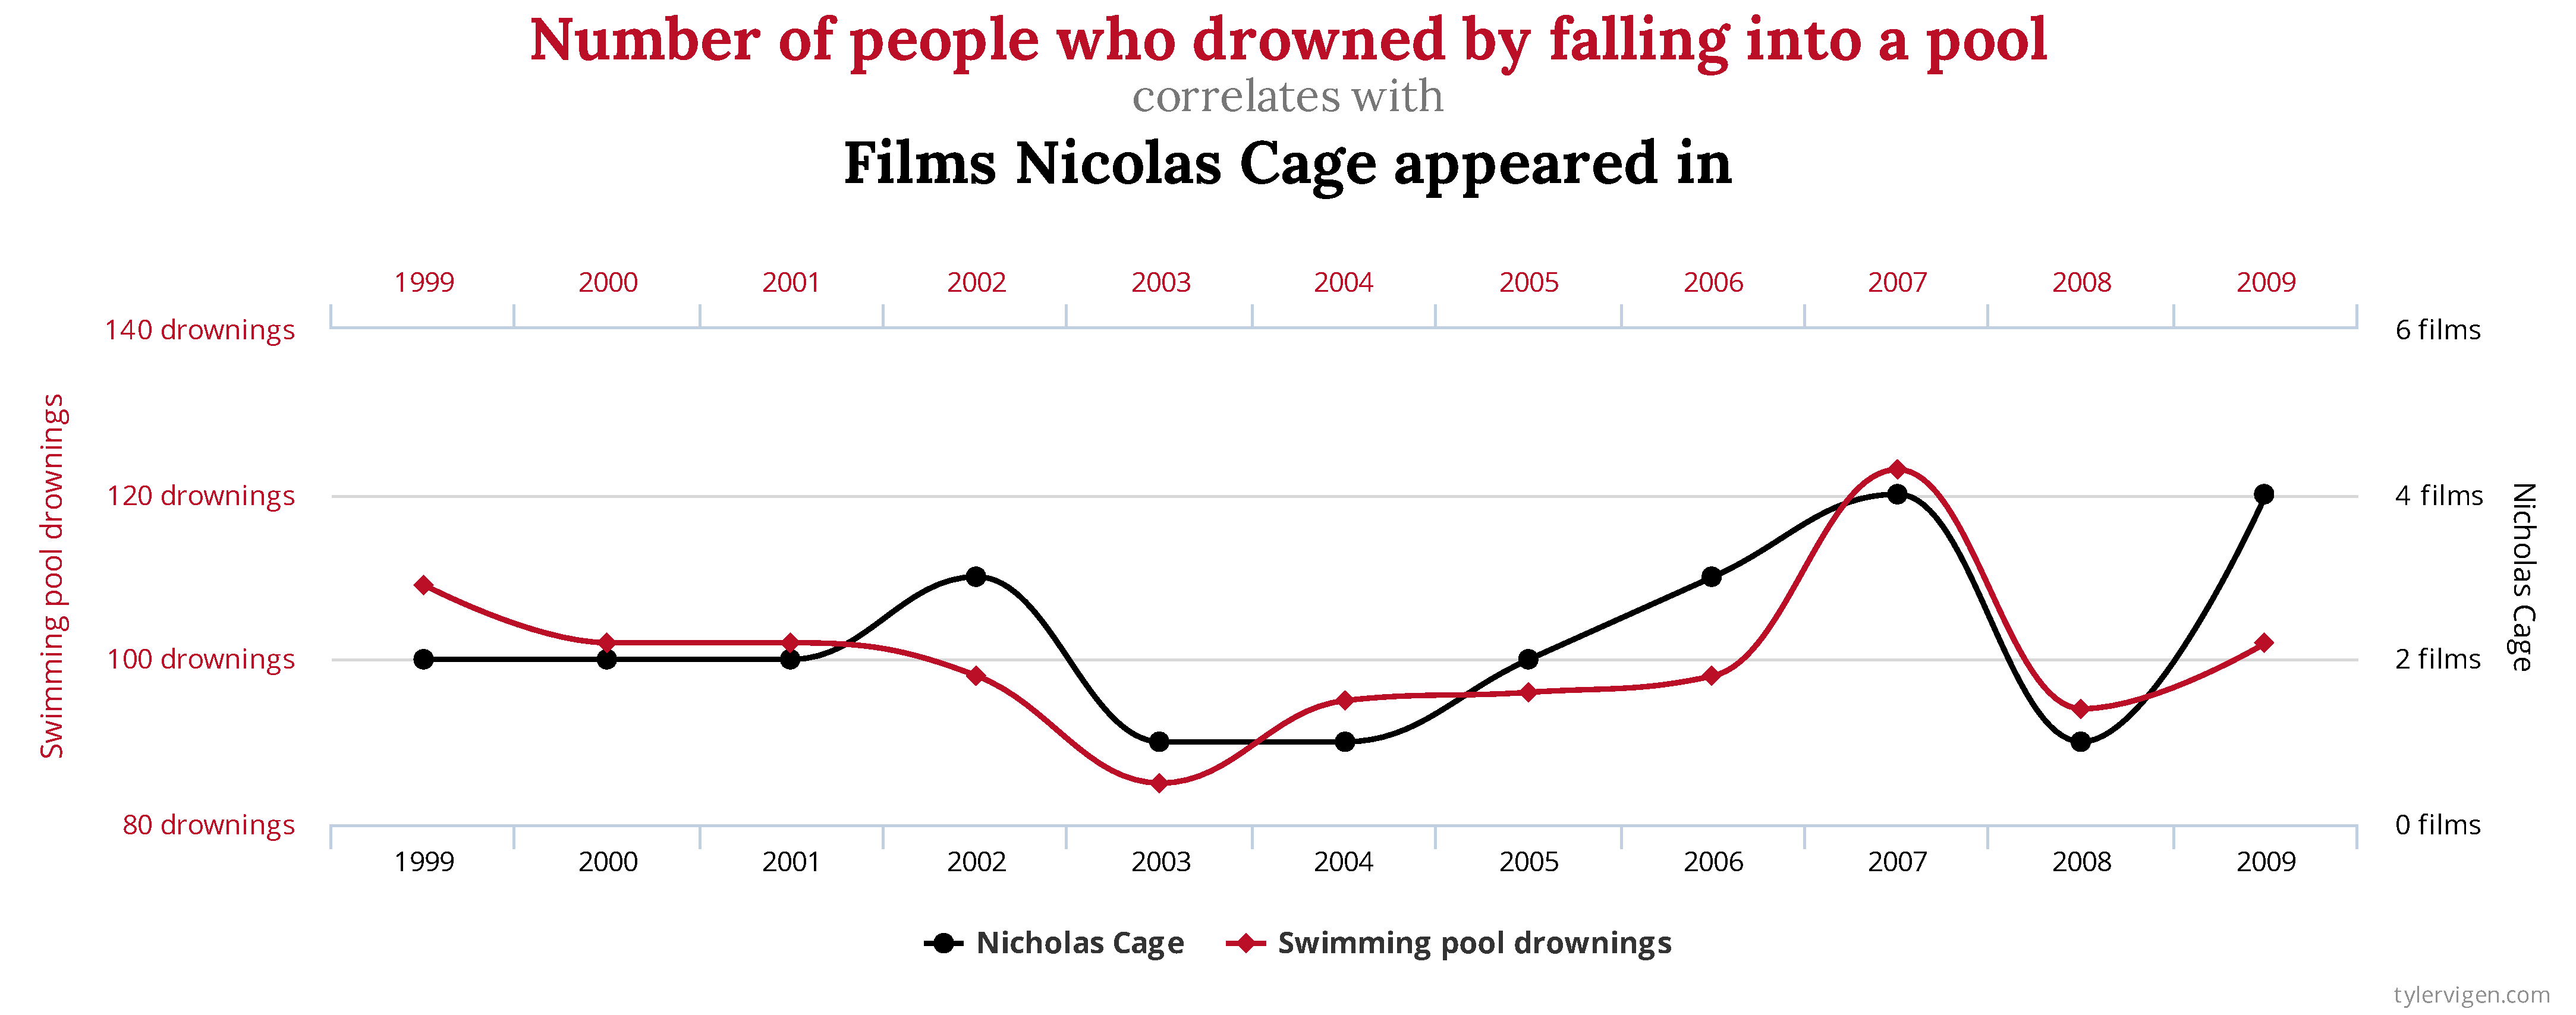
\includegraphics[scale=.23]{pooldiagram.pdf}
%%%%%%%%%%%%%%
%%%%%%%%%%%%%% image from pg 171
%%%%%%%%%%%%%%

These two phenomena vary directly, but it's hard to imagine how they could be causally related.
It's even more difficult to imagine how the following two phenomena could be causally related:

\noindent
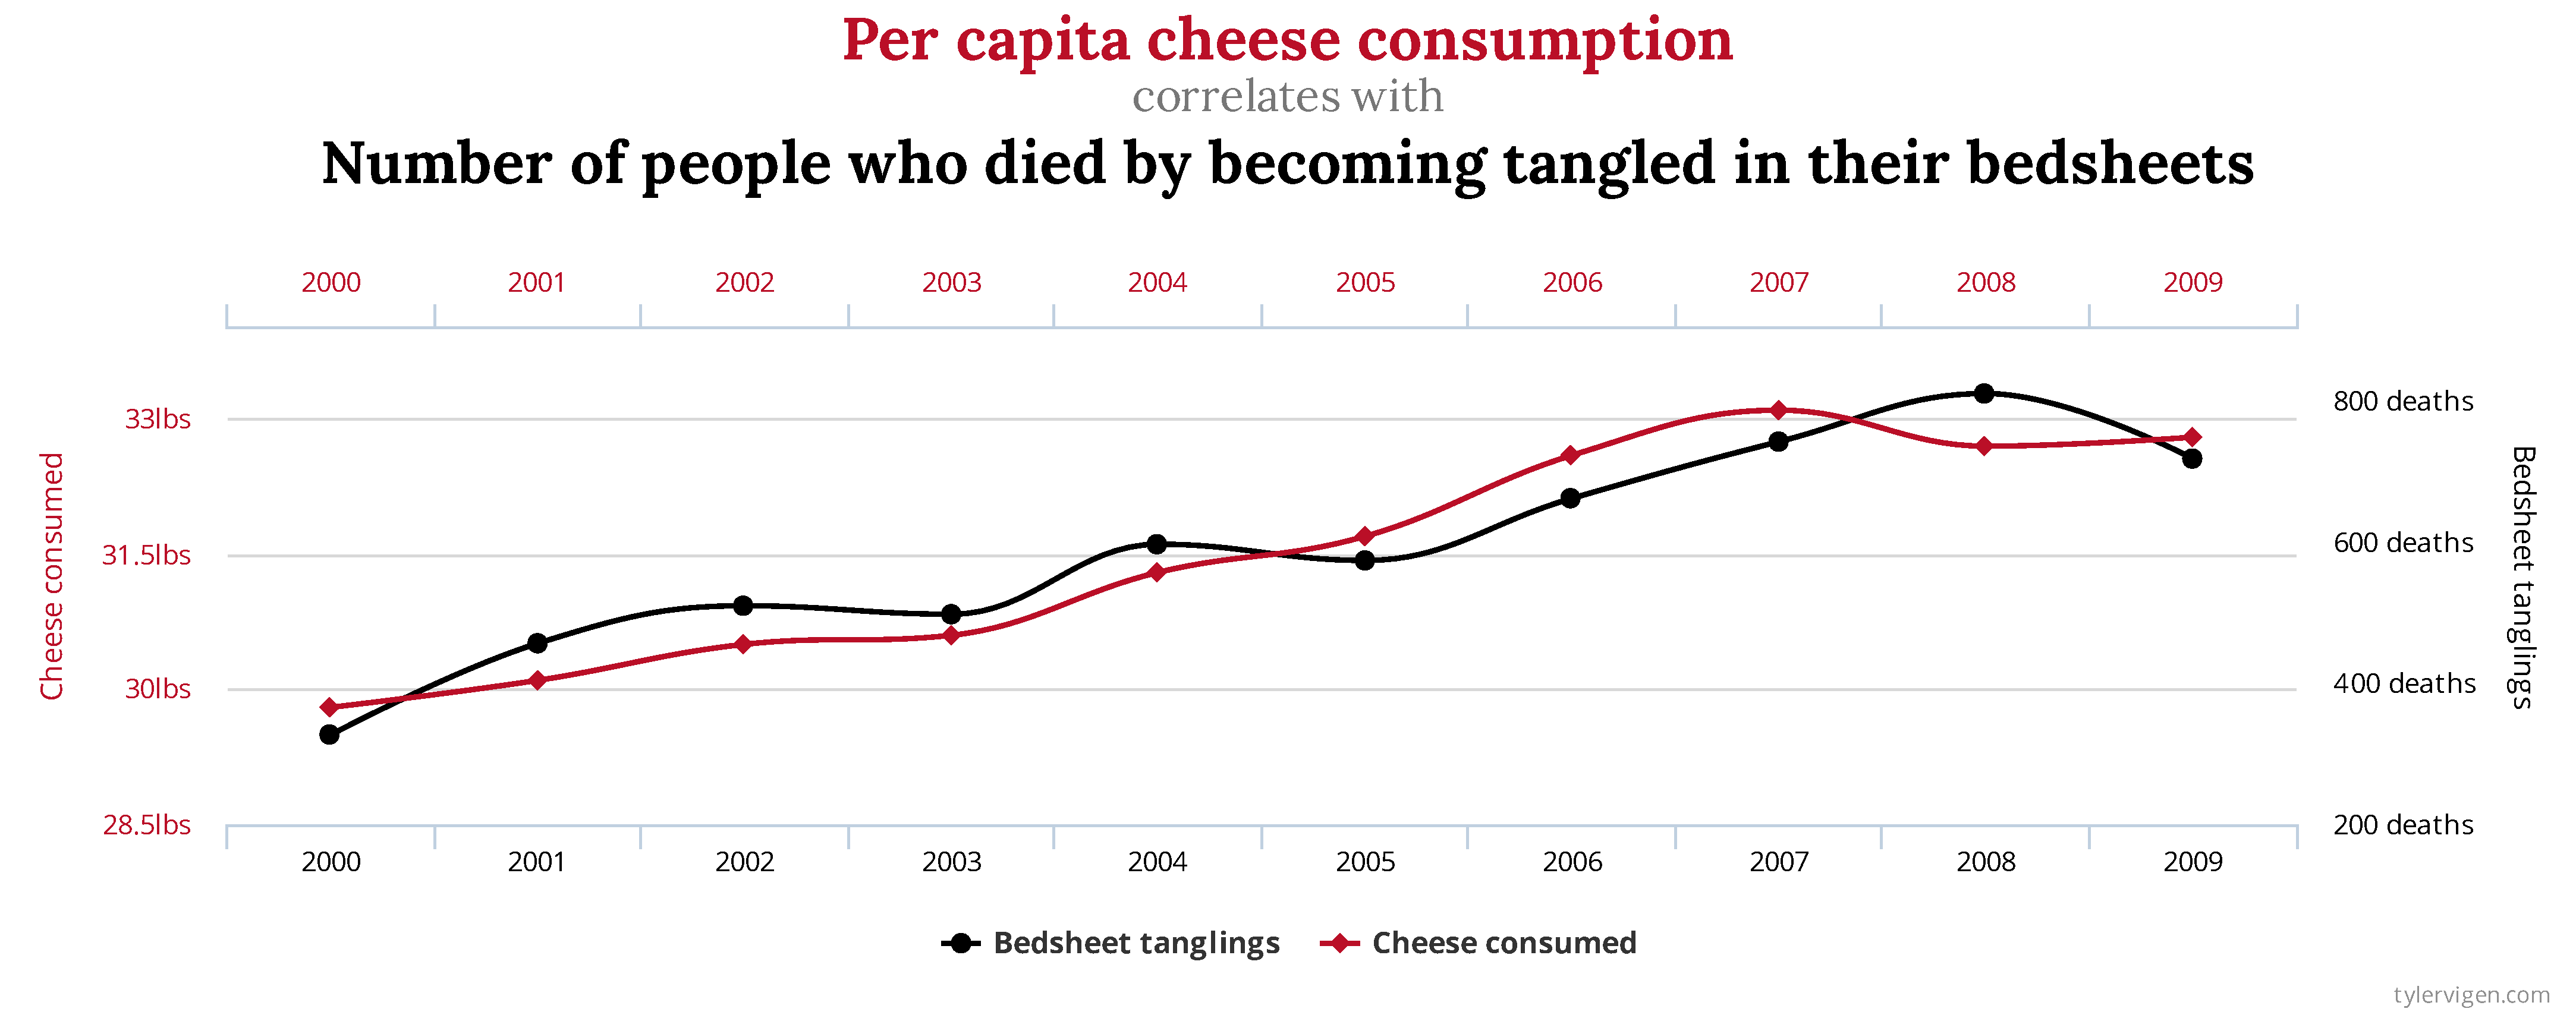
\includegraphics[scale=.23]{cheesediagram.pdf}
%%%%%%%%%%%%%%
%%%%%%%%%%%%%% image from pg 171
%%%%%%%%%%%%%%


So, Mill's Methods can't just be applied willy-nilly; one could end up ``discovering'' causal
connections where none exist. They can provide clues as to potential causal relationships, but care
and critical analysis are required to confirm those results. It's important to keep in mind that the
various methods can work in concert, providing a check on each other. If the drunken logician, for
example, had applied the Method of Difference--removing the 7-Up but keeping everything else
the same--he would have discovered his error (he would've kept getting hangovers). The
combination of the Methods of Agreement and Difference--the Joint Method, the controlled
study--is an invaluable tool in modern scientific research. A properly conducted controlled study
can provide quite convincing evidence of causal connections (or a lack thereof).

Of course, properly conducting a controlled study is not as easy as it sounds. It involves more than
just the application of the Joint Method of Agreement and Difference. There are other potentially
confounding factors that must be accounted for in order for such a study to yield reliable results.
For example, it's important to take great care in separating subjects into the test and control groups:
there can be no systematic difference between the two groups other than the factor that we're
testing; if there is, we cannot say whether the factor we're testing or the difference between the
groups is the cause of any effects observed. Suppose we were conducting a study to determine
whether or not vitamin C was effective in treating the common 
cold.\footnote{Despite widespread belief that it is, researchers have found very little evidence 
to support this claim.}
We gather 100 subjects
experiencing the onset of cold symptoms. We want one group of 50 to get vitamin C supplements,
and one group of 50--the control group--not to receive them. How do we decide who gets placed
into which group? We could ask for volunteers. But doing so might create a systematic difference
between the two groups. People who hear ``vitamin C'' and think, ``yeah, that's the group for me''
might be people who are more inclined to eat fruits and vegetables, for example, and might
therefore be healthier on average than people who are turned off by the idea of receiving vitamin
C supplements. This difference between the groups might lead to different results between the how
their colds progress. Instead of asking for volunteers, we might just assign the first 50 people who
show up to the vitamin C group, and the last 50 to the control group. But this could lead to
differences, as well. The people who show up earlier might be early-risers, who might be healthier
on average than those who straggle in late.

The best way to avoid systematic differences between test and control groups is to randomly assign
subjects to each. We refer to studies conducted this way as randomized controlled studies. And
besides randomization, other measures can be taken to improve reliability. The best kinds of
controlled studies are ``double-blind''. This means that neither the subjects nor the people
conducting the study know which group is the control and which group is receiving the actual
treatment. (This information is hidden from the researchers only while the study is ongoing; they
are told later, of course, so they can interpret the results.) This measure is necessary because of the
psychological tendency for people's observations to be biased based on their expectations. For
example, if the control group in our vitamin C experiment knew they were not getting any
treatment for their colds, they might be more inclined to report that they weren't feeling any better.
Conversely, if the members of the group receiving the vitamin supplements knew that they were
getting treated, they might be more inclined to report that their symptoms weren't as bad. This is
why the usual practice is to keep subjects in the dark about which group they're in, giving a placebo
to the members of the control group. It's important to keep the people conducting the study ``blind''
for the same reasons. If they knew which group was which, they might be more inclined to observe
improvement in the test group and a lack of improvement in the control group. In addition, in their
interactions with the subjects, they may unknowingly give away information about which group
was which via subconscious signals.

Hence, the gold standard for medical research (and other fields) is the double-blind controlled
study. It's not always possible to create those conditions--sometimes the best doctors can do is to
use the Method of Agreement and merely note commonalities amongst a group of patients
suffering from the same condition, for example--but the most reliable results come from such
tests. Discovering causes is hard in many contexts. Mill's Methods are a useful starting point, and
they accurately model the underlying inference patterns involved in such research, but in practice
they must be supplemented with additional measures and analytical rigor in order to yield
definitive results. They can give us clues about causes, but they aren't definitive evidence.
Remember, these are inductive, not deductive arguments. \\

EXERCISES \\

\begin{enumerate}
\item What is meant by the word `cause' in the following--necessary condition, sufficient condition,
or mere tendency?
\begin{enumerate}
\item (a) Throwing a brick through a window causes it to break.
\item (b) Slavery caused the American Civil War.
\item (c) Exposure to the cold causes frostbite.
\item (d) Running causes knee injuries.
\item (e) Closing your eyes causes you not to be able to see.
\end{enumerate}
\item Consider the following scenario and answer the questions about it:
\begin{itemize}
\item Alfonse, Bertram, Claire, Dominic, Ernesto, and Francine all go out to dinner at a local
greasy spoon. There are six items on the menu: shrimp cocktail, mushroom/barley soup,
burger, fries, steamed carrots, and ice cream. This is what they ate:
\end{itemize}
\begin{itemize}
\item Alfonse: shrimp, soup, fries
\item Bertram: burger, fries, carrots, ice cream
\item Claire: soup, burger, fries, carrots
\item Dominic: shrimp, soup, fries, ice cream
\item Ernesto: burger, fries, carrots
\item Francine: ice cream
\end{itemize}
\begin{itemize}
\item That night, Alfonse, Claire, and Dominic all came down with a wicked case of foodpoisoning. The others felt fine.
\end{itemize}
\begin{enumerate}
\item (a) Using only the Method of Agreement, how far can we narrow down the list of possible
causes for the food poisoning?
\item (b) Using only the Method of Difference, how far can we narrow down the list of possible
causes for the food poisoning?
\item (c) Using the Joint Method, we can identify the cause. What is it?
\end{enumerate}
\item For each of the following, identify which of Mill's Methods is being used to draw the causal
conclusion.
\begin{enumerate}
\item (a) A farmer noticed a marked increase in crop yields for the season. He started using a
new and improved fertilizer that year, and the weather was particularly ideal--just enough
rain and sunshine. Nevertheless, the increase was greater than could be explained by these
factors. So he looked into it and discovered that his fields had been colonized by
hedgehogs, who prey on the kinds of insect pests that usually eat crops.
\item (b) I've been looking for ways to improve the flavor of my vegan chili. I read on a website
that adding soy sauce can help: it has lots of umami flavor, and that can help compensate
for the lack of meat. So the other day, I made two batches of my chili, one using my usual
recipe, and the other made exactly the same way, except for the addition of soy sauce. I
invited a bunch of friends over for a blind taste test, and sure enough, the chili with the soy
sauce was the overwhelming favorite!
\item (c) The mere presence of guns in circulation can lead to higher murder rates. The data are
clear on this. In countries with higher numbers of guns per capita, the murder rate is higher;
and in countries with lower numbers of guns per capita, the murder rate is correspondingly
lower.
\item (d) There's a simple way to end mass shootings: outlaw semiautomatic weapons. In 1996,
Australia suffered the worst mass shooting episode in its history, when a man in Tasmania
used two semiautomatic rifles to kill 35 people (and wound an additional 19). The
Australian government responded by making such weapons illegal. There hasn't been a
mass shooting in Australia since.
\item (e) A pediatric oncologist was faced with a number of cases of childhood leukemia over a
short period of time. Puzzled, he conducted thorough examinations of all the children, and
also compared their living situations. He was surprised to discover that all of the children
lived in houses that were located very close to high-voltage power lines. He concluded that
exposure to electromagnetic fields causes cancer.
\item (f) Many people are touting the benefits of the so-called ``Mediterranean'' diet because it
apparently lowers the risk of heart disease. Residents of countries like Italy and Greece, for
example, consume large amounts of vegetables and olive oil and suffer from heart
problems at a much lower rate than Americans.
\item (g) My daughter came down with what appeared to be a run-of-the-mill case of the flu:
fever, chills, congestion, sore throat. But it was a little weird. She was also experiencing
really intense headaches and an extreme sensitivity to light. Those symptoms struck me as
atypical of mere influenza, so I took her to the doctor. It's a good thing I did! It turns out
she had a case of bacterial meningitis, which is so serious that it can cause brain damage if
not treated early. Luckily, we caught it in time and she's doing fine.
\end{enumerate}
\end{enumerate}
